\begin{savequote}[75mm] 
Nulla facilisi. In vel sem. Morbi id urna in diam dignissim feugiat. Proin molestie tortor eu velit. Aliquam erat volutpat. Nullam ultrices, diam tempus vulputate egestas, eros pede varius leo.
\qauthor{Quoteauthor Lastname} 
\end{savequote}

\chapter{The title of chapter one}

- radiotherapia oggi (vs surgery and chemio) - serve fonte

- serve fonte, ho usato katia parodi

Results of radiotherapy are improved when a high dose of radiation with highbiological effectiveness is delivered to the tumor with the least possible dose to the sorrounding tissues, especially in the case of critical organs.
In order to increase the conformity of the dose delivered to the tumor, diverse technologies have been considered and used.
Traditional forms of radiotherapy, X-ray tubes (energy $\sim$ 100 keV) or radioactive isotopes have been replaced by linear accelerators delivering $\sim$ 10 MeV from different directions (e.g. Intensity Modulated Radio Therapy), and provide treatment with photons and electrons.
Though being widely used as a standard in radiation therapy, the effectiveness of conventional electromagnetic radiation is limited by the intrinsic characteristics of interaction with matter.
In particular two aspects unfavours in principle the usability of electromagnetic radiation with respect to ion for tumor targeting: the depth dose profile, which does not allow for an optimal dose deposition to the tumor sparing vital organs
and the inferior biological efeffectiveness, which is the limiting factor in case of radioresistant tumors.
Heavier charged particles, like protons and ions (He-Ca) have the potentiality to overcome the limits of convetional therapy With respect to this, the scientific community is directing his attention towards possible improvements of ion beam therapy.

- qui citare entervision website

The work outlined in these pages have been sponsored by  The European training network in digital medical imaging for radiotherapy (ENTERVISION) at the European Center of Nuclear Research (CERN). ENTERVISION was established in February 2011 in response to the critical need for reinforcing research in online 3D digital imaging and the training of professionals in order to deliver some of the key elements and building blocks for realizing the vision for early detection and more precise treatment of tumours.

\section{Hadrontherapy}
\subsection{Ion beam therapy}

The first proposition of ion beam therapy was presented in 1946 by R. Wilson. The original idea was exploit the physical properties of ion interaction in matter to improve the precision in radiotherapy treatments.  
Making use of the so called Bragg peak, that is using the fact that protons and ions in general deposit a maximum of energy at the end of their trajectory, the treatment could save the sorrounding tissue from radiation overdose.

The dose deposited by photons, considered as the gold standard for tumor treatment, is maximum close to the beginning of the trajectory in the body and is characterized by an exponential decrease. As a consequence an undesired radiation dose is delivered to healthy tissues around the targeted tumor.

The recent therapeutic interest of ions in the field of radiotherapy relies mainly on their high relative biological effectiveness.
LET (linear energy transfer) has long been viewed as the main parameter to discern the biological effect of different kinds of radiation. It is a measure for the energy deposited by a charged particle traveling through matter. LET is closely related to stopping power and is not a constant value, since it changes along the particle's path (es 10 kEV/um for gamma, 100 kev/um for protons, 1000 kev/um for ions).
When considering ions of different atomic number LET becomes a limited parameter to evaluate the biological effect. In this sense the relative biological effectiveness (RBE) is considered the most accurate quantity, since it is defined as the biological effect of one type of ionizing radiation relative to another, given the same amount of absorbed energy. As the charge of the incident ions increases, so does the probability of severe DNA damage. An elevate RBE in the Bragg peak region has clearly been demonstrated for ions heavier than Helium.
As a consequence they prove to be more effective for targeting radioresistant or inoperable tumors.

\subsection{Beam delivery}

Ion beams are delivered by either cyclotrons or synchrotrons. In the first case the beam has a fixed energy which is tuned by means of degraders in order to deliver the correct dose profile. In the case of syncrotron the beam is delivered in spills and the energy is varied between spills. In the case of Carbon only syncrhotrons can be used.
To deliver the dose to the planned target volume (PTV) different energies are superimposed in order to obtain the so-called spread-out Bragg peak (SOBP). The beam is usually deliverd in a passive beam shaping setup or a scanning system. 

Different sources of error can worsen the dose delivery profile, such as patient mispositioning and evolution of the tumor/morpology of the patient. In addition the complex physics of ion interaction leads to  imprecisions in the treatment plannings, due to fragmentation of the incident beam and range uncertainties.

Usually treatment planning systems cope with these problems by irradiating a volume larger than the tumor itself, called planning target volume (PTV) which contains the CTV. Complex compensating systems, including x-ray imaging techniques and patient positiong systems, allow to reduce errors in the dose profiles delivered.
The dose delivered by a ion beam system is much more sensitive to these deviations than the one delivered by a photon beam. Due to the high biological effectiveness of ion beams wrong ranges could lead to dramatic underdosage to the tumor or overdosage to organ at risk sorrounding.

\subsection{Monitoring of the beam}

- correlation b+ activity

\section{Positron Emission Tomography}
\subsection{Principles}

\subsection{TOFPET}

\section{Outline of the thesis}
\section{MEDICAL PHYSICS - HIGH ENERGY}
\subsection{CERN}
\subsection{Time profiles}



$x = 1/\alpha$ 

\cite{Eigen1971, Knuth1968}

$$\zeta = \frac{1039}{\pi}$$

Fig.~\ref{fig:myFullPageFigure}.

\begin{figure}  
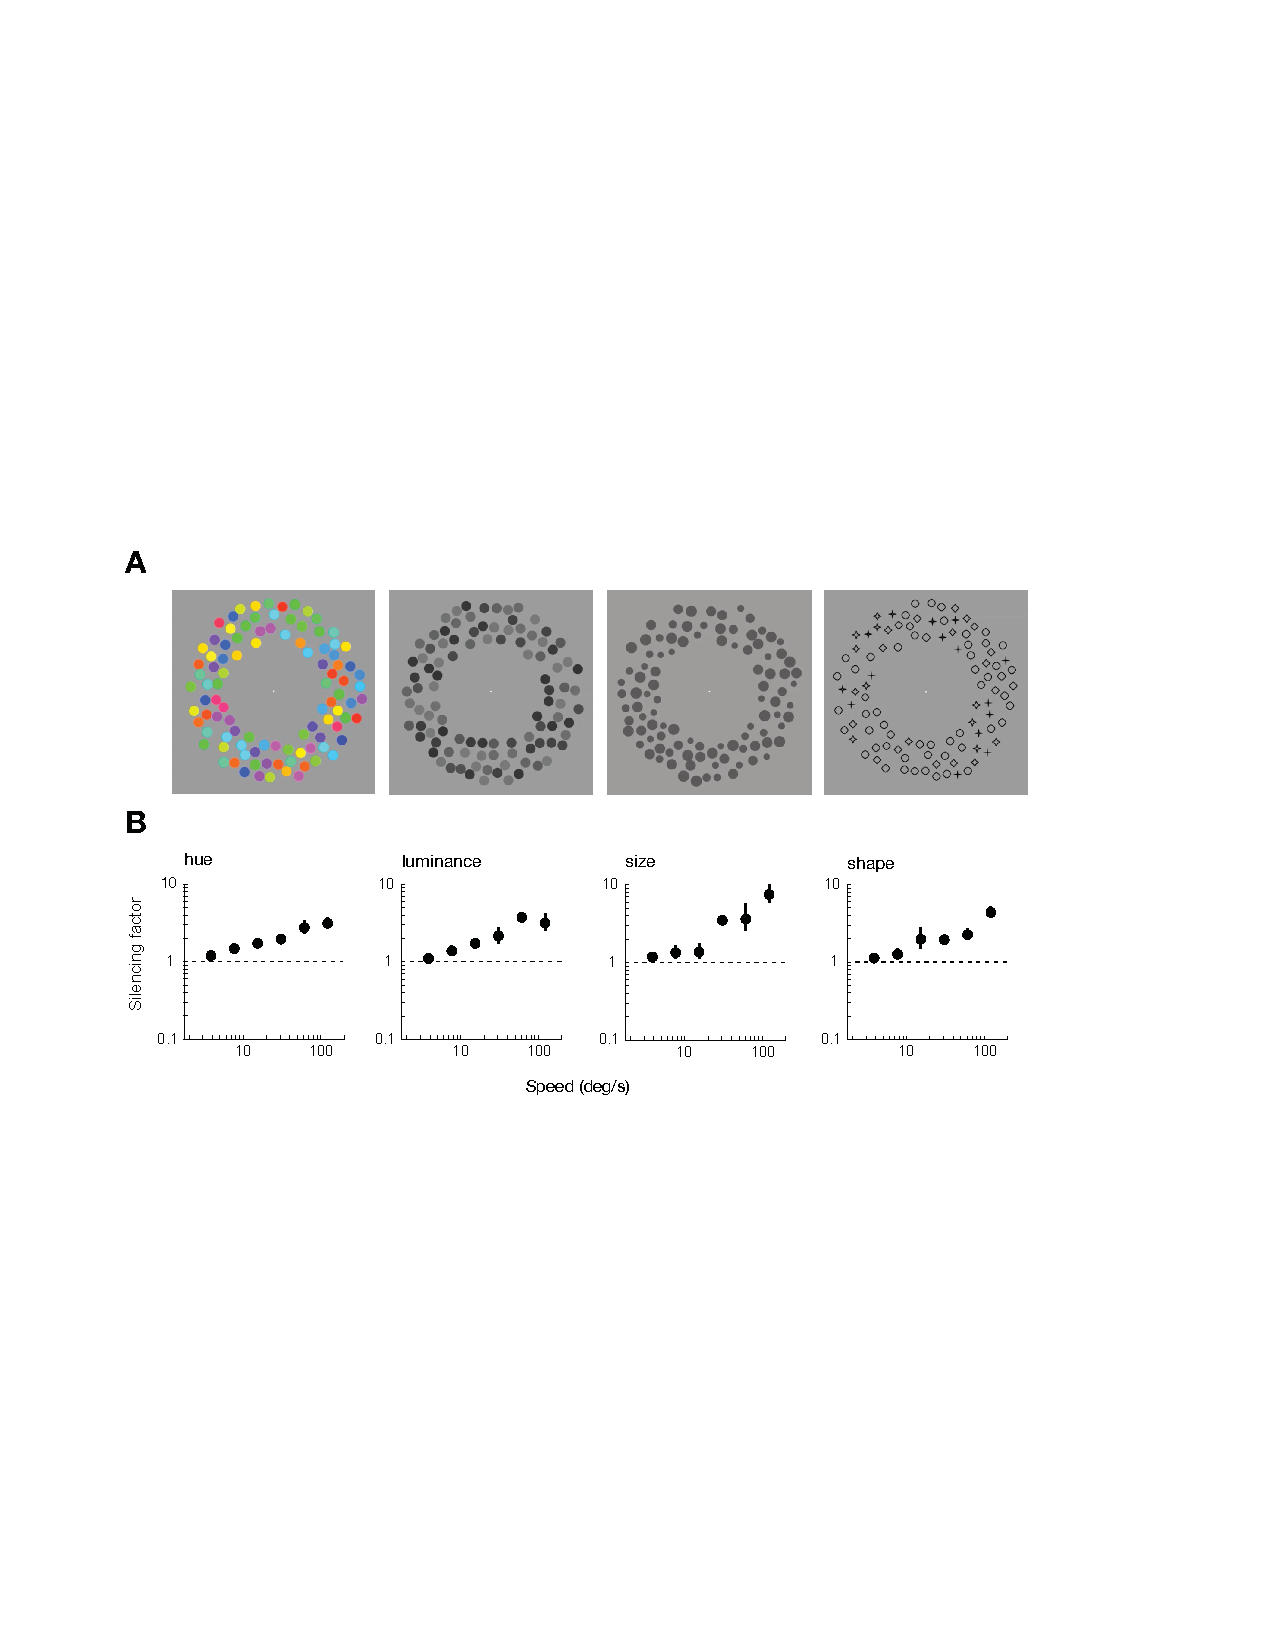
\includegraphics[width=\textwidth]{figures/fig1}
\caption[Short figure name.]{This is a figure that floats inline and here is its caption.
\label{fig:myInlineFigure}}
\end{figure}

\afterpage{\clearpage}


